% !TeX spellcheck = es_ANY
% Chapter 1

%\chapter{Chapter Title Here} % Main chapter title
%
%\label{Chapter1} % For referencing the chapter elsewhere, use \ref{Chapter1} 

%----------------------------------------------------------------------------------------

% Define some commands to keep the formatting separated from the content 
\newcommand{\keyword}[1]{\textit{#1}}
%\newcommand{\tabhead}[1]{\textbf{#1}}
%\newcommand{\code}[1]{\texttt{#1}}
%\newcommand{\file}[1]{\texttt{\bfseries#1}}
%\newcommand{\option}[1]{\texttt{\itshape#1}}

%----------------------------------------------------------------------------------------

\section{Introducción}
	La termodinámica es el estudio de las transformaciones de energía, en la etapa más temprana de esta rama de las ciencias, se pensaba que el calor era una clase de fluido cuya cantidad neta en el universo permanecía siempre constante. El aumento de temperatura de un objeto era explicado a partir de la migración de calor de un objeto a otro \cite{feynman2011feynman, fermi1986}. Usando esta teoría del calor como fluido, el ingeniero Sadi Carnot dio origen a la termodinámica con el análisis del problema, sobre cómo generar el mejor y más eficiente motor de vapor en 1824. Posteriormente, Julius von Mayer en 1842 descubrió una equivalencia entre calor y trabajo mecánico, también publicado por James Joule el siguiente año \cite{fermi1986}. A raíz de esto hoy se considera el calor como una forma de energía que puede ser convertida a energía mecánica, eléctrica, lumínica, etc. \cite{fermi1986}.
	
	Los resultados de la termodinámica se encuentran implícitos en una serie de declaraciones que reciben el nombre de leyes de la termodinámica, las cuales nos permiten conocer la dirección natural en la que tienen lugar los cambios químicos y físicos en la materia \cite{atkins2011physical}. Históricamente la termodinámica fue desarrollada antes que se tuviera un entendimiento sobre la estructura interna de la materia, además, sus leyes tampoco siguen un orden cronológico \cite{feynman2011feynman}. La primera ley surge del trabajo realizado por Mayer en 1842, una de las leyes más importantes de la ciencia en general: la conservación de la energía \cite{feynman2011feynman, fermi1986}. La segunda se atribuye a Carnot y Clausius en 1824, y habla sobre la reversibilidad de los procesos \cite{feynman2011feynman}.
	
	A pesar que el estudio de las transformaciones de energía parece un tema distante de la química, la termodinámica, estudiada a través de la fisicoquímica, ha demostrado ser de vital importancia tanto en la química como la biología \cite{atkins2011physical}. No sólo permite entender la producción o consumo de energía en las reacciones químicas, además constituye una herramienta fundamental para responder preguntas que se encuentran en el corazón de la bioquímica, por ejemplo sobre cómo fluye la energía en una célula, y qué tan grande puede ser la agrupación de moléculas que forman estructuras complejas como las células \cite{atkins2011physical}. En otros casos, por ejemplo, existen propiedades de fácil determinación para un analista, como el color, masa y densidad. Sin embargo existen propiedades que dependen de los enlaces, estructura molecular y naturaleza del material, entre estas se encuentran propiedades termodinámicas de interés químico: capacidad calorífica, entalpía, entropía, etc \cite{gaisford2016principles}.
	
	\newpage
	
	Dentro de la fisicoquímica, el estudio y medición de las transferencias de energía en forma de calor se denomina calorimetría, y constituye una de las áreas más viejas de esta rama de la química \cite{zielenkiewicz2006theory}. Se podría considerar que la historia de esta comienza en junio de 1783, con la presentación de \textit{Memoria del calor} (Mémoire de la Chaleur) por Lavoisier y Laplace a la Academia Francesa \cite{zielenkiewicz2006theory}. Empíricamente todos los procesos físicos y químicos están acompañados de absorción o liberación de energía en forma de calor. Lo anterior hace de la calorimetría una técnica con un amplio rango de aplicaciones \cite{wadso2001standards}. Entre estas aplicaciones se tienen titulaciones, flujos, reacciones y estudio de procesos de sorción \cite{gaisford2016principles}.
	
	El instrumento para realizar este tipo de mediciones se denomina calorímetro, y existen de diversos tipos. Pueden ser clasificados por el tipo de condiciones que imponen al sistema, por ejemplo, volumen constante, temperatura constante, calor constante, etc. Estos calorímetros reciben el nombre de: bombas calorimétricas, isotérmicos, y adiabáticos, correspondientemente \cite{gaisford2016principles, wadso2001standards}. También pueden ser clasificados por el principio de funcionamiento, si compensan los flujos de energía o los acumulan \cite{gaisford2016principles}. Finalmente, dependiendo del rango de las potencias medidas, se tienen dos términos comúnmente usados: \keyword{microcalorimetría} para el caso de experimentos realizados en el rango de los microvatios \cite{wadso2001standards, wadso2003new}, mientras que para escalas de nanovatios son usados \keyword{nanocalorímetros} \cite{wadso2003new}.
	
	En particular el trabajo a realizar busca armar, poner en marcha y calibrar un microcalorímetro \texttt{2277 Thermal Activity Monitor}. Esto implica un entendimiento del funcionamiento del calorímetro a nivel interno, desde las partes mecánicas, la etapa electrónica y los principios fisicoquímicos detrás del mismo. En este proyecto, por su naturaleza, se hace imperativo que una vez alcanzado el nivel de operación del calorímetro, se realice una calibración para constatar que el funcionamiento es correcto y concuerda con los resultados obtenidos por la literatura así como con un microcalorímetro moderno disponible en el grupo de investigación \textit{\groupname}.
	
\section{Objetivos}
	\subsection{Objetivo general}
		Entregar al grupo de investigación de \groupname\ el calorímetro \texttt{2277 Thermal Activity Monitor} con el que se cuenta, en funcionamiento y calibrado para su uso en las investigaciones activas del grupo.
		
	\subsection{Objetivos específicos}
		\begin{itemize}
			\item Ensamblar el equipo \texttt{2277 Thermal Activity Monitor}.
			\item Realizar el cableado y conexiones electrónicas pertinentes al mismo.
			\item Calibración eléctrica, determinación de las señales de entrada y salida, flujo de las bombas hidráulicas y temperatura del baño.
			\item Calibración química, determinación de la potencia disipada por la hidrólisis lenta de un líquido al fluir por la celda experimental.
		\end{itemize}

\section{Justificación del proyecto}
	En general la calorimetría permite una gran variedad de análisis, muchos de ellos cuentan con aplicaciones industriales, comerciales, biológicas y químicas, permitiendo el entendimiento de las interacciones moleculares en soluciones \cite{blandamer1998titration}. Una ventaja de la calorimetría es que no es específica, ni invasiva además de no es sensible a las propiedades electroquímicas y ópticas de un sistema dado, siendo esto de vital importancia para las investigaciones de procesos biológicos, el estudio del crecimiento bacteriano y para la detección de compuestos biológicos \cite{winkelmann2004application}. Por otro lado la calorimetría también permite el estudio de la termodinámica en sistemas de absorción, bien sea por la universalidad de la absorción física en las superficies como catalizadores, o en procesos industriales como la separación de mezclas de gases \cite{morrison1987calorimetry}. Finalmente la calorimetría es el método clásico para la determinación de propiedades termodinámicas en las muestras, entre estas se encuentran la capacidad calorífica, la entalpía, entropía y energía libre de Gibbs, las cuales constituyen el punto de partida de gran cantidad de estudios teóricos, desarrollos y producción industrial de un compuesto químico \cite{wang2005determination, gaisford2016principles}.

	El calorímetro \texttt{2277 Thermal Activity Monitor} con el que cuenta el grupo de investigación se encuentra desarmado, a la espera de su ensamble y puesta en funcionamiento. Este instrumento permite monitorear una gran variedad de reacciones químicas y bioquímicas, lo anterior debido a su capacidad de cuantificar procesos exotérmicos y endotérmicos. Estas reacciones pueden ser estudiadas en el rango de 5 - 80 $^\circ$C \cite{Suurkuusk}. Este rango de temperaturas se debe a el uso de un baño termostatado de 25 litros. Cuatro balones de medición independientes se encuentran sumergidos en este baño, permitiendo medidas con desviaciones de temperatura inferiores a $\pm2\times10^{-4}$ $^\circ$C, alcanzando de esta manera medidas en el rango de microvatios \cite{Suurkuusk}. Es por esta razón que poner en marcha y calibrar el equipo con el que cuenta el grupo de investigación resulta una contribución importante para el mismo así como para el \deptname\ en general.
	
\section{Metodología}
	Para el ensamble del calorímetro se cuenta con el catálogo de partes, y el manual de instrucciones. En el primero se detallan y enumeran las partes del equipo, en la \autoref{fig:partes} se muestran ejemplos de los distintos sistemas con los que el calorímetro cuenta \cite{Suurkuusk}. 
	
	\begin{figure}[h]
		\centering
		\begin{subfigure}[b]{0.3\textwidth}
			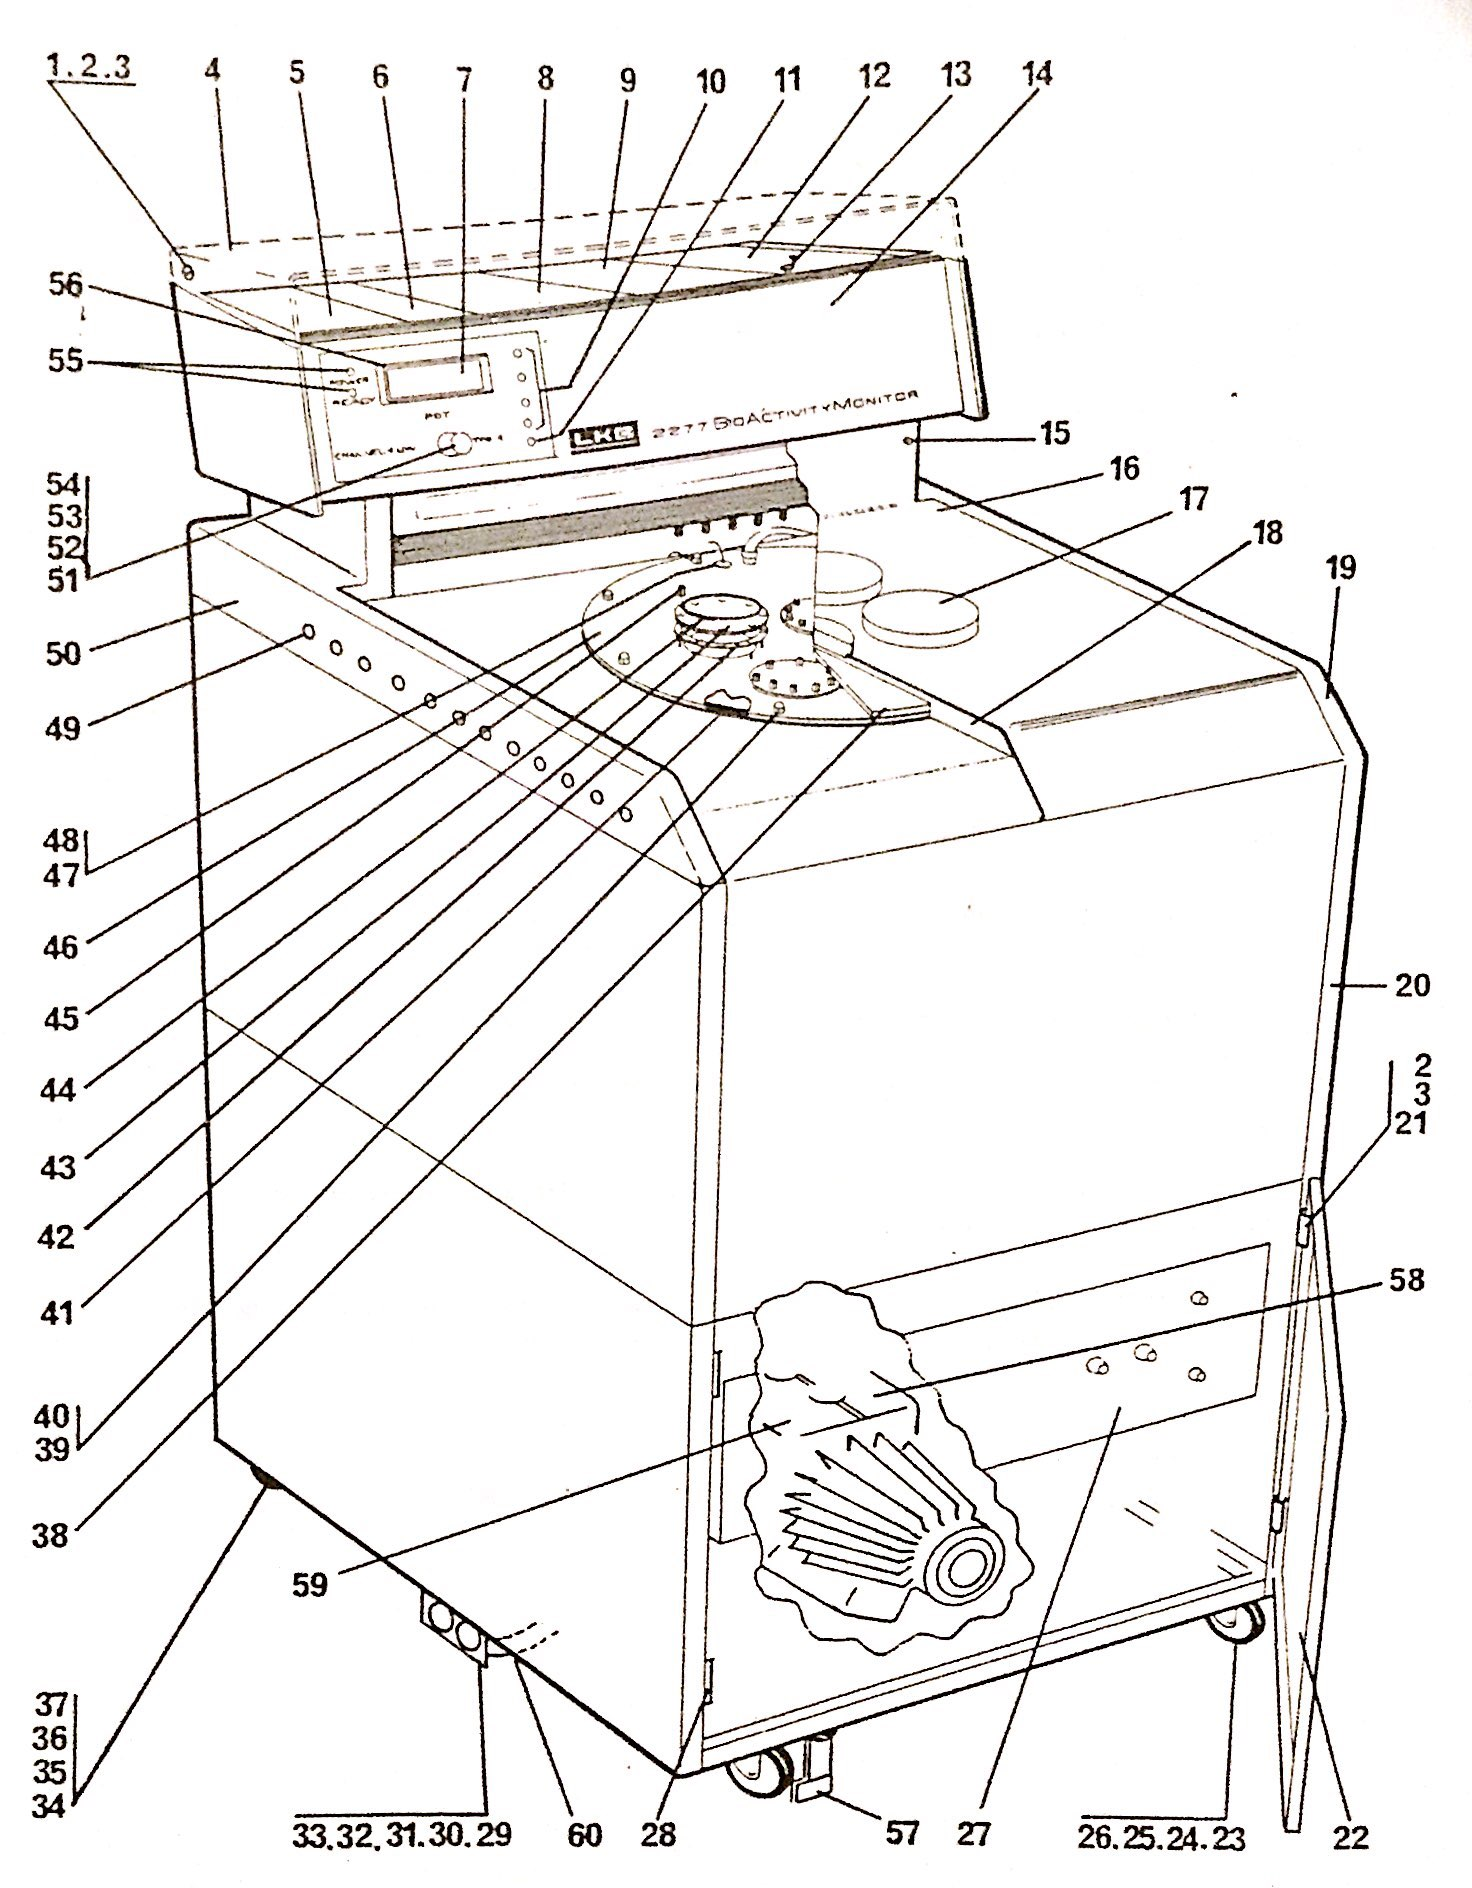
\includegraphics[width=\textwidth]{Figures/images_1.jpg}
			\caption{Vista exterior del equipo con sus componentes.}
			\label{fig:vistaExterior}
		\end{subfigure}
		~ 
		\begin{subfigure}[b]{0.37\textwidth}
			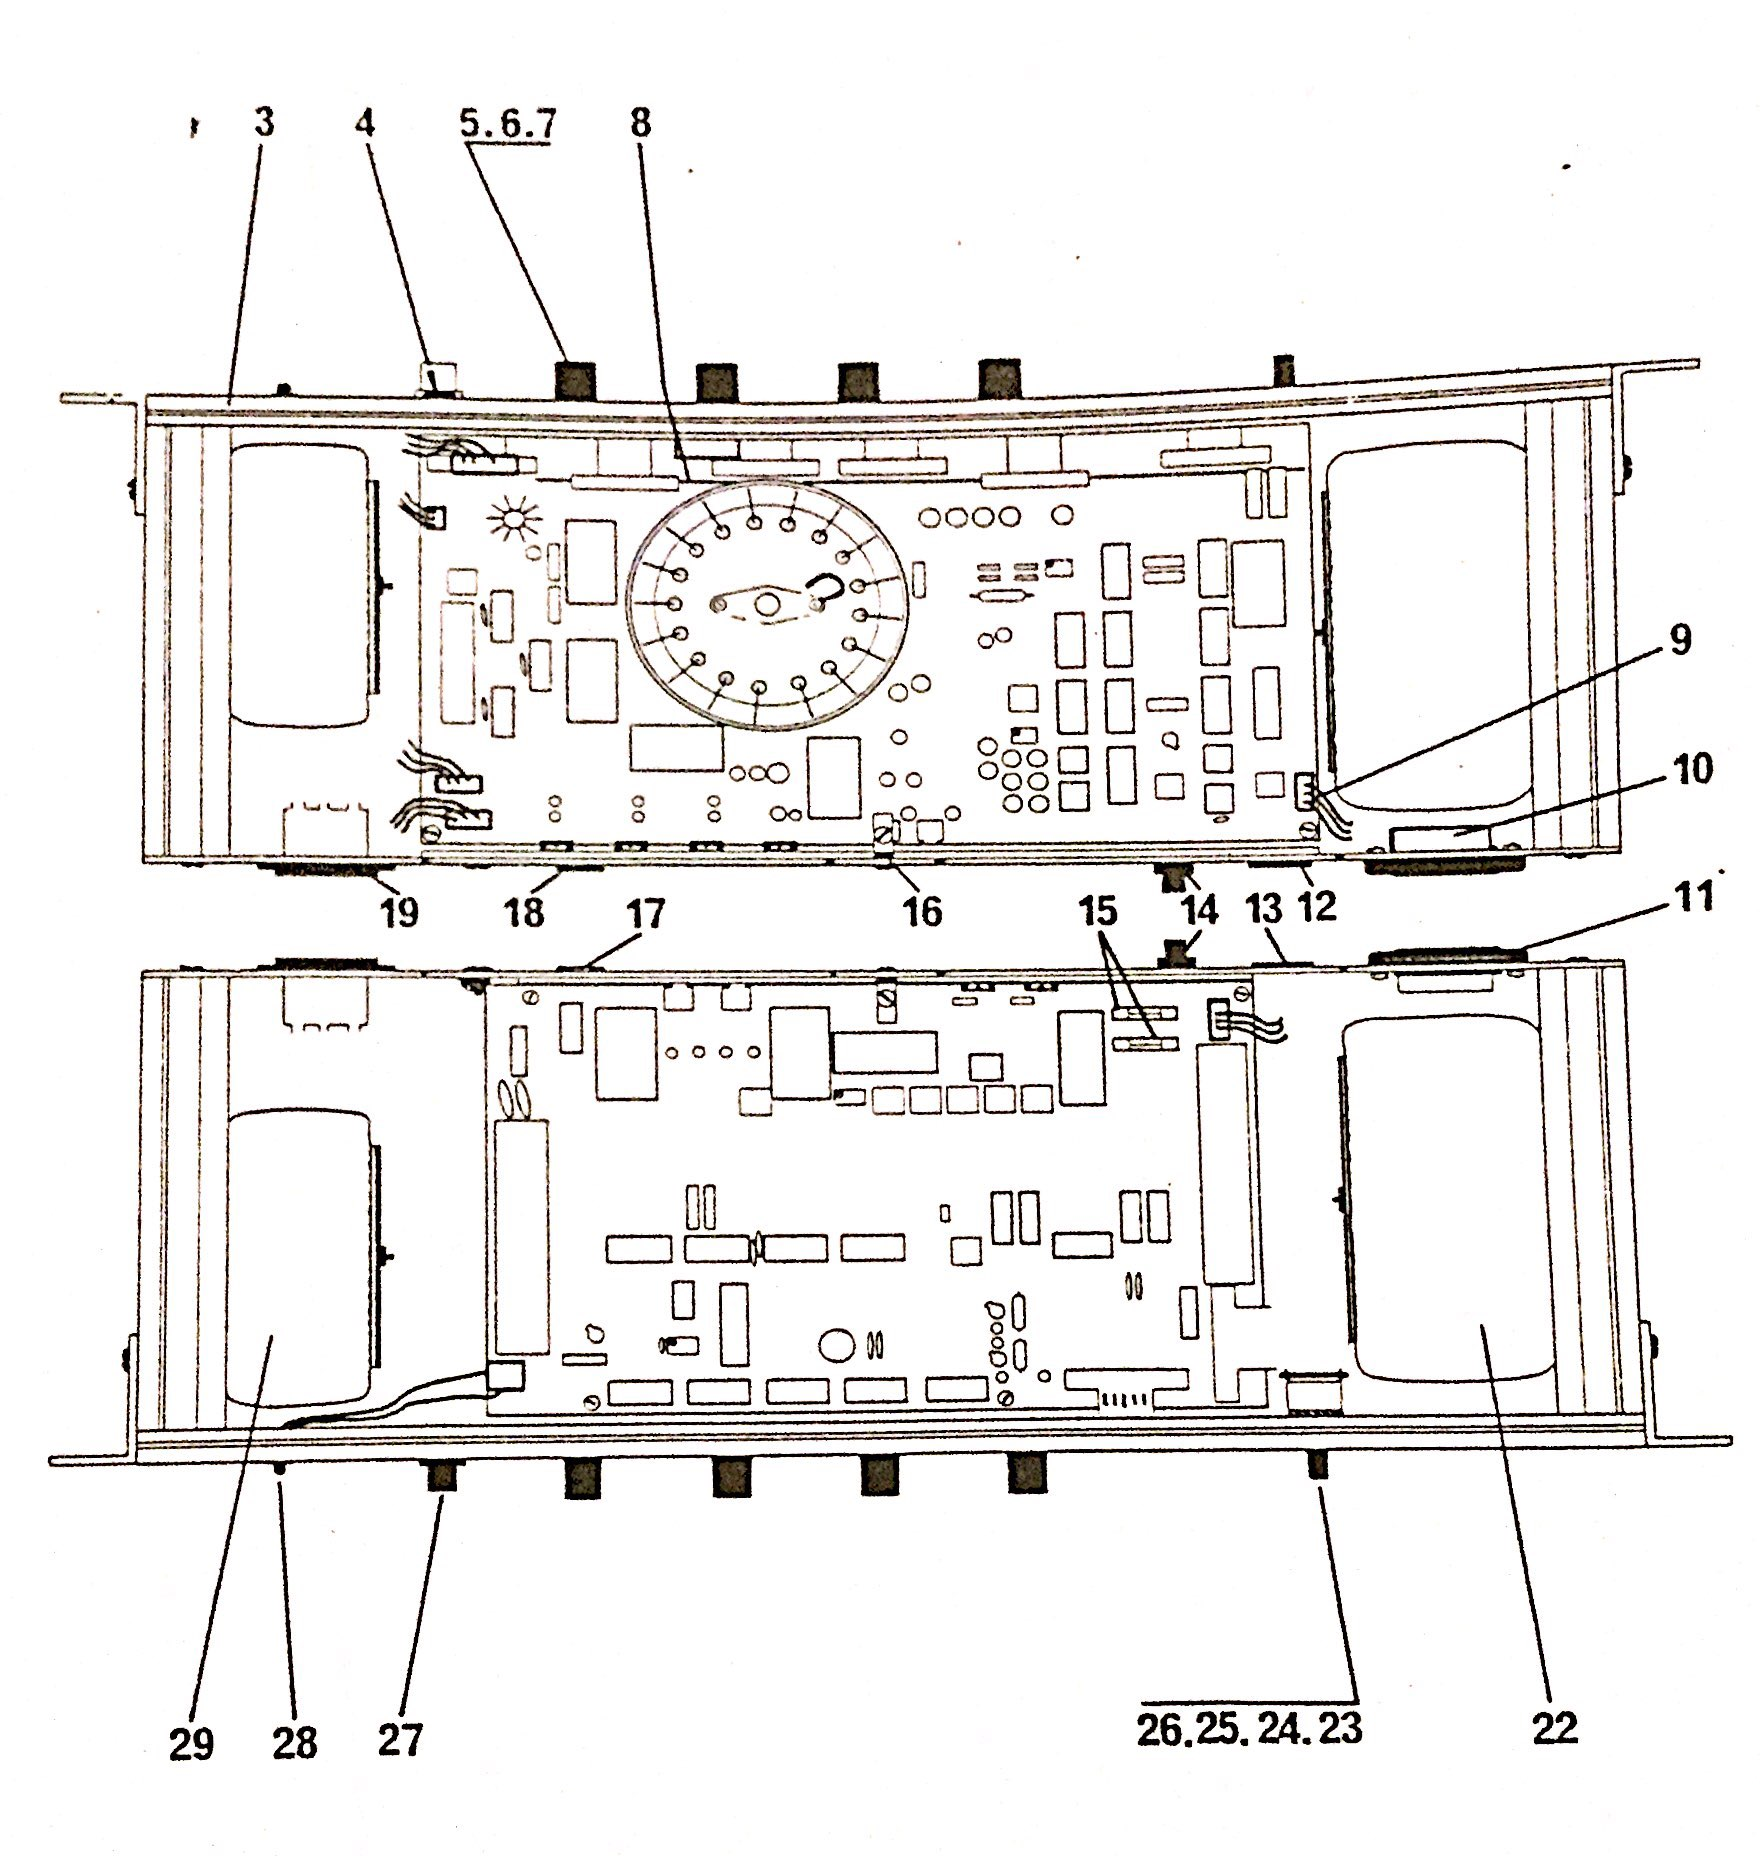
\includegraphics[width=\textwidth]{Figures/images_2.jpg}
			\caption{Parte del sistema eléctrico del calorímetro.}
			\label{fig:sistemaElectrico}
		\end{subfigure}
		~ 
		\begin{subfigure}[b]{0.25\textwidth}
			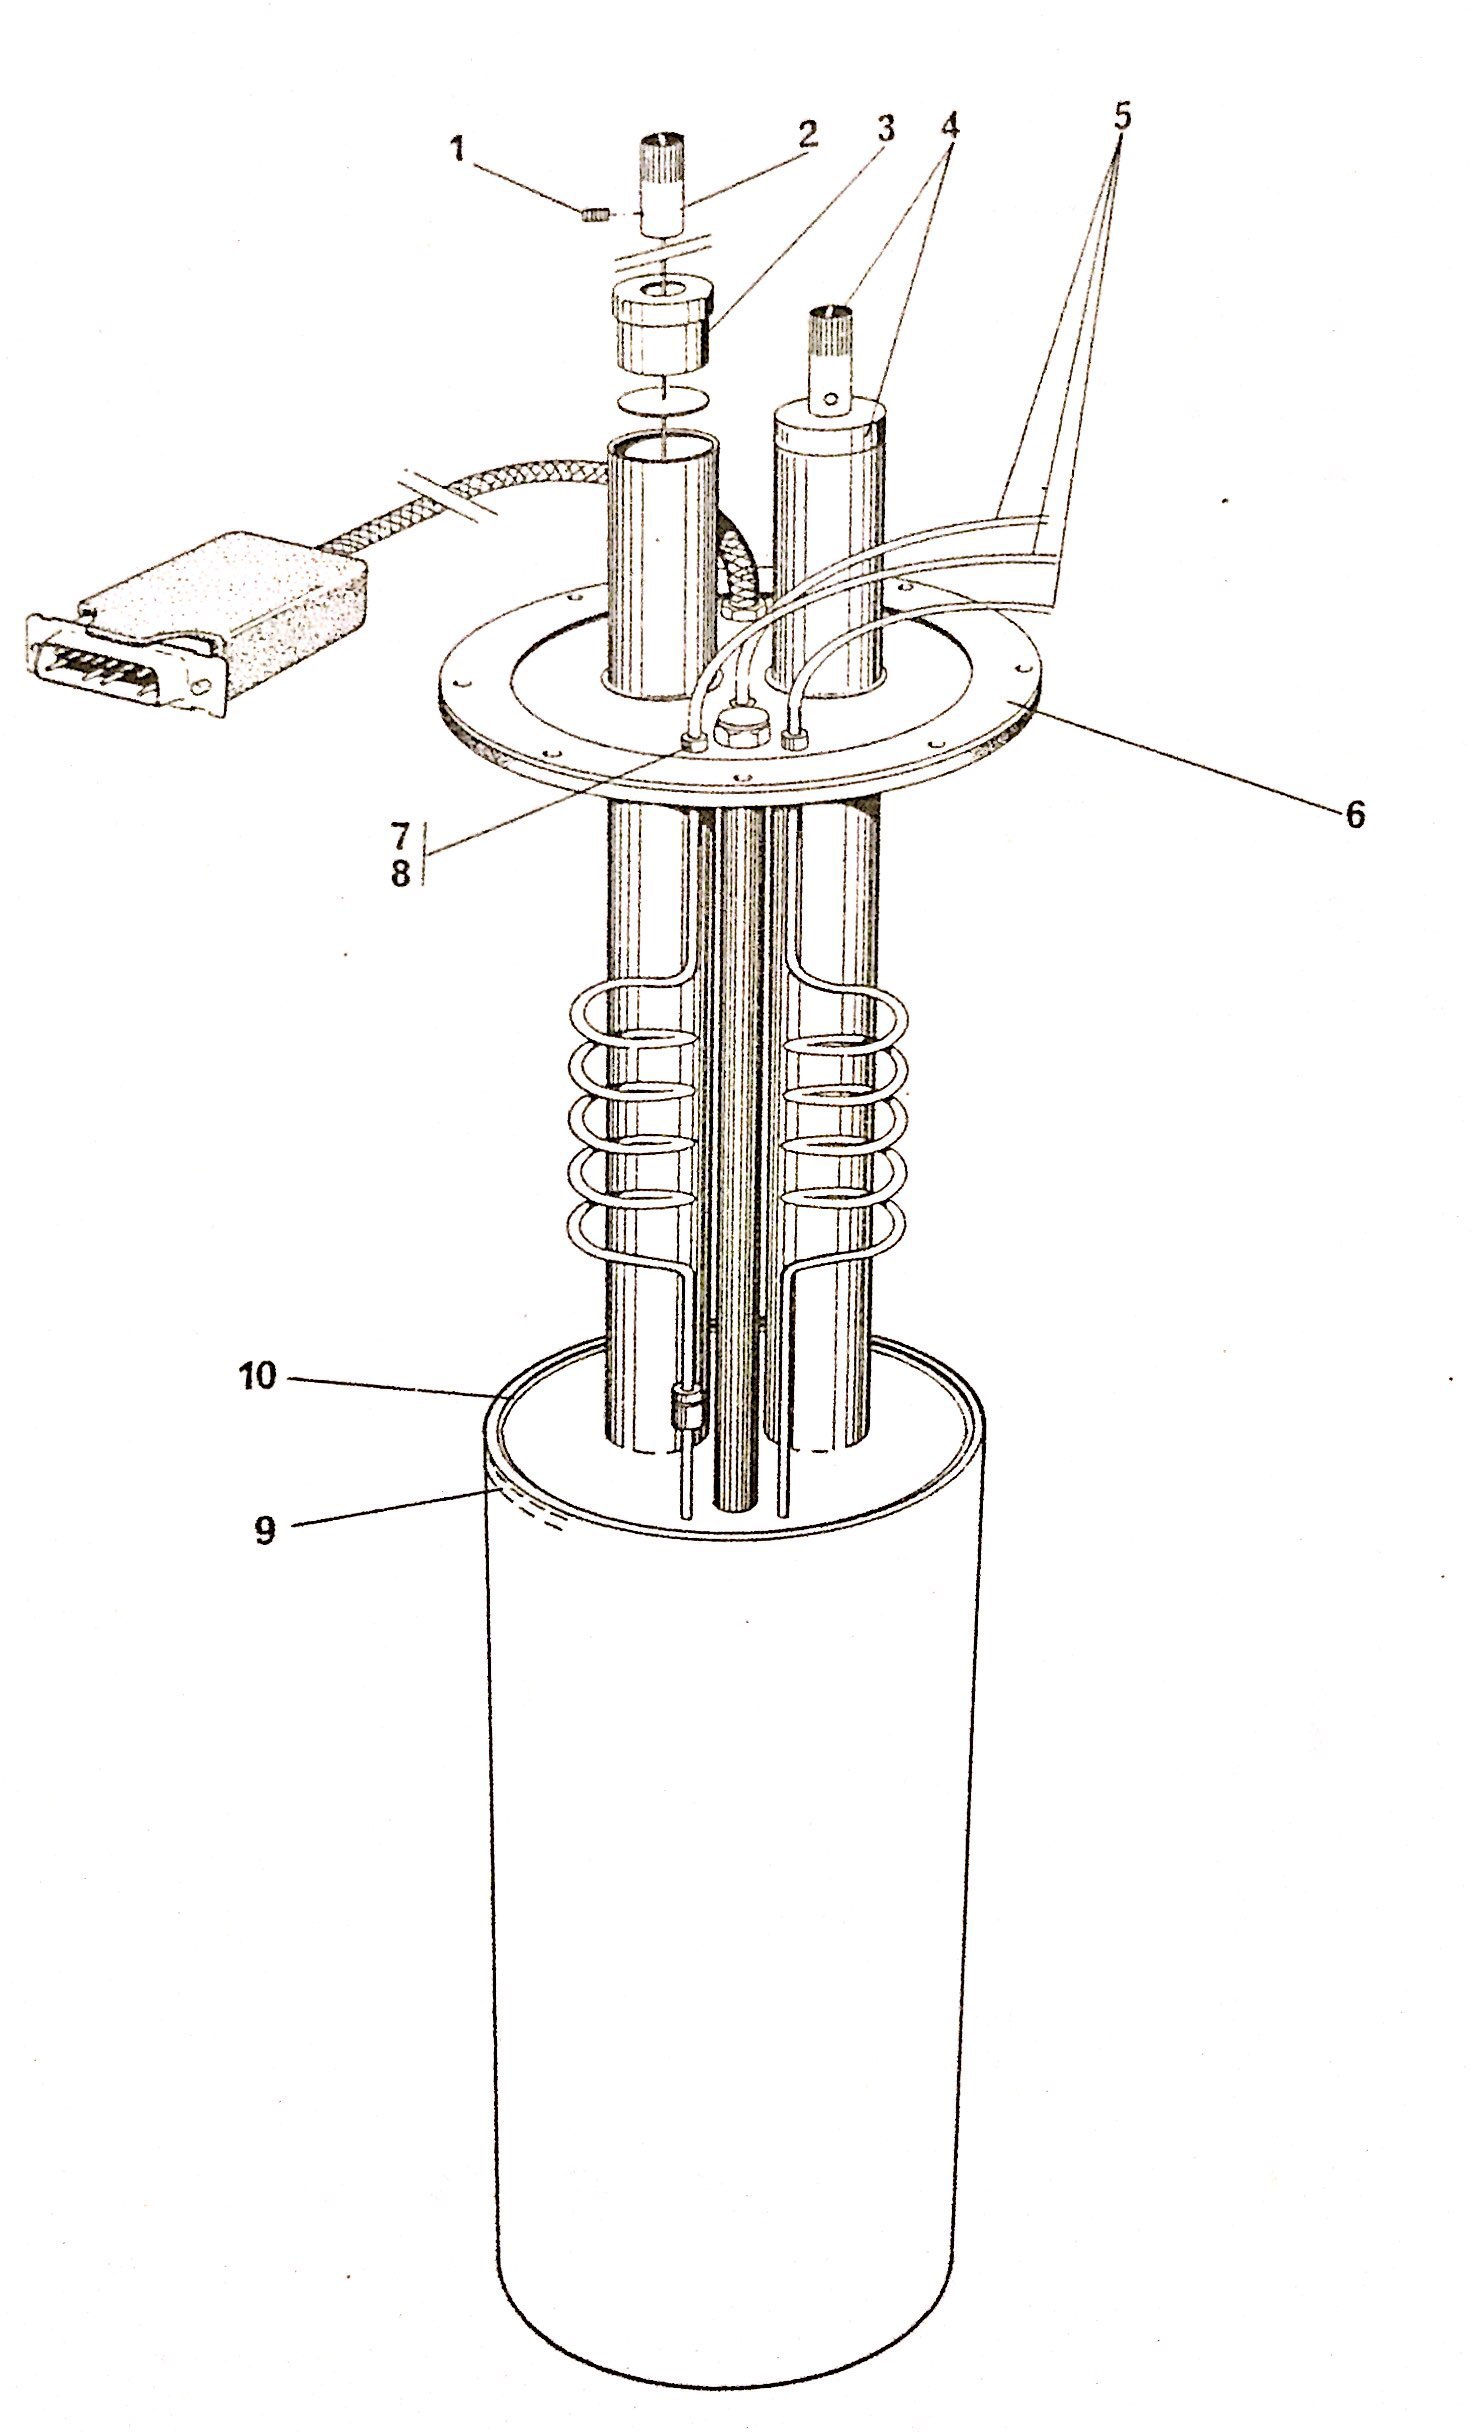
\includegraphics[width=\textwidth]{Figures/images_3.jpg}
			\caption{Celda de medición.}
			\label{fig:celda}
		\end{subfigure}
		\caption{text}
		\label{fig:partes}
	\end{figure}
	Usando esta información se llevará a cabo el ensamble del calorímetro así como las conexiones eléctricas.	A nivel electrónico, la liberación o absorción de energía térmica se mide usando una celda Peltier, las cuales tienen una respuesta proporcional en voltaje, de esta forma se obtiene una señal eléctrica a partir de pequeñas variaciones de temperatura en la celda de reacción. La señal eléctrica es procesada por el sistema digital del instrumento \cite{Suurkuusk}. De esta forma es posible realizar una calibración eléctrica del sistema.
	
	
	
\newpage

\section{Cronograma}
	\begin{table}[h]
		\centering
		\caption{Cronograma de actividades}
		\label{tb: cronograma}
		\footnotesize
		\begin{tabular}{|c|c|c|c|c|c|c|c|c|c|c|c|c|c|c|c|c|}
			\hline
			\rowcolor[HTML]{C0C0C0} 
			\cellcolor[HTML]{C0C0C0}                                       & \multicolumn{16}{c|}{\cellcolor[HTML]{C0C0C0}\textbf{Semana}} \\ \cline{2-17} 
			\rowcolor[HTML]{EFEFEF} 
			\multirow{-2}{*}{\cellcolor[HTML]{C0C0C0}\textbf{Actividades}} & \textbf{1} & \textbf{2} & \textbf{3} & \textbf{4} & \textbf{5} & \textbf{6} & \textbf{7} & \textbf{8} & \textbf{9} & \textbf{10} & \textbf{11} & \textbf{12} & \textbf{13} & \textbf{14} & \textbf{15} & \textbf{16} \\ \hline
			\cellcolor[HTML]{EFEFEF}
			\textbf{Revisión bibliográfica} & x & x & x & & & & x & x & x & x & & & & x & x & x \\ \hline
			\cellcolor[HTML]{EFEFEF}\textbf{Revisión de manuales} & x & x & x & x & & & & & & & & & & & & \\ \hline
			\cellcolor[HTML]{EFEFEF}\textbf{Ensamble del equipo} & x & x & x & x & & & & & & & & & & & & \\ \hline
			\cellcolor[HTML]{EFEFEF}\textbf{Cableado y electrónica} & & & x & x & x & x & & & & & & & & & & \\ \hline
			\cellcolor[HTML]{EFEFEF}\textbf{Calibración eléctrica} & & & & & & x & x & x & & & & & & & & \\ \hline
			\cellcolor[HTML]{EFEFEF}\textbf{Calibración química} & & & & & & & & & x & x & x & x & & & & \\ \hline
			\cellcolor[HTML]{EFEFEF}\textbf{Análisis de datos} & & & & & & & & & & & x & x & x & & & \\ \hline
			\cellcolor[HTML]{EFEFEF}\textbf{Elaboración del documento} & & & & & & & x & x & x & x & & & & x & x & x \\ \hline
			\cellcolor[HTML]{EFEFEF}\textbf{Presentación del proyecto} & & & & & & & & & & & & & & & & x \\ \hline
		\end{tabular}
	\end{table}

\section{Presupuesto}
	 El grupo de investigación en \groupname\ además del \deptname\ cuentan con los insumos (reactivos, disolventes, materiales, y equipos) necesarios para el desarrollo del proyecto y los análisis requeridos por el mismo.
	 
	 %Tabla 2. Presupuesto aproximado para el desarrollo del trabajo de grado.
	 %Materiales
	 %Justificación
	 %Valor COP ($)
	 %Reactivos: 4-dimetilaminosalicilaldehído, POCl3, acetoacetato de etilo, 2-cloropiridina, sal de indolinio.
	 %Obtención de los intermedios y el producto final.
	 %2.000.000
	 %Disolventes: DMF, DCM, EtOH, MeOH, AcOEt, tolueno, CDCl3, DMSO-d6.
	 %Medio de reacción, purificación y caracterización mediante UV-vis, fluorescencia, RMN y HRMS.
	 %1.500.000
	 %Servicios técnicos: RMN, HRMS, UV-vis, fluorescencia, rayos X
	 %Uso las técnicas de caracterización de intermediarios y producto final.
	 %2.000.000
	 %Total
	 
	 %5.500.000
	 

\section{Consideraciones éticas}
	La metodología del proyecto requiere de pocos reactivos químicos, ninguno de los cuales implica cuidados especiales más allá de la correcta disposición final de los mismos. En el desarrollo de la propuesta no se requieren equipos que representen ningún tipo de riesgo. Por otro lado, el resultado de la tesis será un equipo de laboratorio en funcionamiento y calibrado, lo anterior es considerado como la generación de una herramienta, sin ninguna consideración ética especial.